\documentclass{beamer}
\usepackage{ctex} %中文字体设置
% \usetheme{Copenhagen}
\usetheme{Madrid}
\title{基于xxx的xxxx研究}
% \subtitle{An Engineer's Perspective}
\author{作者姓名}
\institute[] % (optional)
{
%	\inst{1}%
广东省xxx中心\\
xxxx重点实验室\\
  华南理工大学
	\and
%	\inst{2}%
%	Faculty of Chemistry\\
%	Very Famous University
}
\date{2023年10月13日}
\usepackage{mathtools}
\usepackage{color}
\usepackage{graphics}
\usepackage{hyperref}
\usepackage{listings}

\usepackage{caption}
\captionsetup{font={scriptsize}}
\usepackage{graphicx}
\usepackage{float} 
\usepackage{subfig}

% package to build the theorem-like environments
\usepackage{amsthm} 
% set a new style for remark environments
\theoremstyle{remark}
\newtheorem*{remark}{Remark}


% \logo{
\includegraphics[height=2cm]{2.jpeg}}
\usepackage{tikz}
% \logo{\tikz\node[opacity=.2,inner sep=0pt] {
\includegraphics[scale=0.2]{1.jpeg}};}

\usepackage{beamerfoils}
\MyLogo{\tikz\node[opacity=.2,inner sep=0pt] {
\includegraphics[scale=0.15]{1.jpeg}};} 
% \MyLogo{
\includegraphics[height=0.7cm]{1.jpeg}} %\vspace是 向上移动\vspace*{8.5cm}
% 如果还需要向左移动11cm , 在后面添加\hspace{11cm},完整语句如下
% \MyLogo{\vspace*{8.5cm}\includegraphics[height=0.7cm]{NDC-sign.png} \hspace{11cm}} 

% logo of my university
\titlegraphic{
\includegraphics[width=2.2cm]{2.jpeg}
}

% Adapted from beamerinnerthemedfault.sty
% set the itemize item symbol as a diamond
\setbeamertemplate{itemizeitem}{\scriptsize$\diamond$}
% set the itemize subitem symbol as a triangle
\setbeamertemplate{itemize subitem}{\scriptsize$\blacktriangleright$}
% set the itemize subsubitem symbol as a circle with a dot
\setbeamertemplate{itemize subsubitem}{\scriptsize$\odot$}


\AtBeginSubsection[]
{
	\begin{frame}
		\frametitle{目录}
		\tableofcontents[currentsubsection]
	\end{frame}
}

\begin{document}
\LogoOff  % 标题页不显示logo

\begin{frame}
\titlepage
\end{frame}
\LogoOn % 以下显示logo

\begin{frame}
\frametitle{目录}
\tableofcontents
\end{frame}

\section{立题依据}

\subsection{研究意义}


\begin{frame}
	\frametitle{多智能体系统}
	\begin{itemize}
		\item 多智能体系统由若干彼此相互通信的具有一定计算、自主决策及运动能力的个体组成,这些个体被称为智能体,如无人机、智能小车等。
			\begin{itemize}
				\item 受自然界群体行为所启发。
				\item Reynolds规则(1987):避碰,速度匹配,聚集。
				\item 代数图论、稳定性理论为主要工具。
			\end{itemize}
	\end{itemize}
	\begin{figure}[htbp]
		\centering
		\begin{minipage}[c]{0.5\textwidth} 
				\centering
				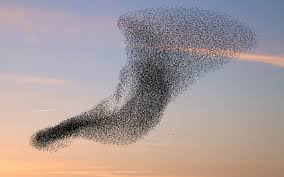
\includegraphics[width=0.8\linewidth]{Fig/f1.jpeg}
				\caption{鸟群}
		\end{minipage}%
		\begin{minipage}[c]{0.5\textwidth}
				\centering
				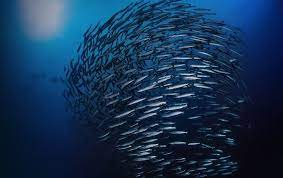
\includegraphics[width=0.8\linewidth]{Fig/f2.jpeg}
				\caption{\label{}鱼群}
		\end{minipage}
	\end{figure}		
\end{frame}

\begin{frame}
	\frametitle{编队控制}
	\begin{itemize}
		\item 作为多智能体系统研究的一个热点问题,编队控制指多个智能体组成的团队 在向特定目标或方向运动的过程中,相互之间保持预定的几何形态 (即队形),同 时又要适应环境约束 (例如避开障碍) 的控制问题。
		\item 在军事、航天、工业、娱乐等各个领域具有广阔的应用前景
	\end{itemize}
	\begin{figure}[htbp]
		\centering
		\begin{minipage}[c]{0.33\textwidth} 
				\centering
				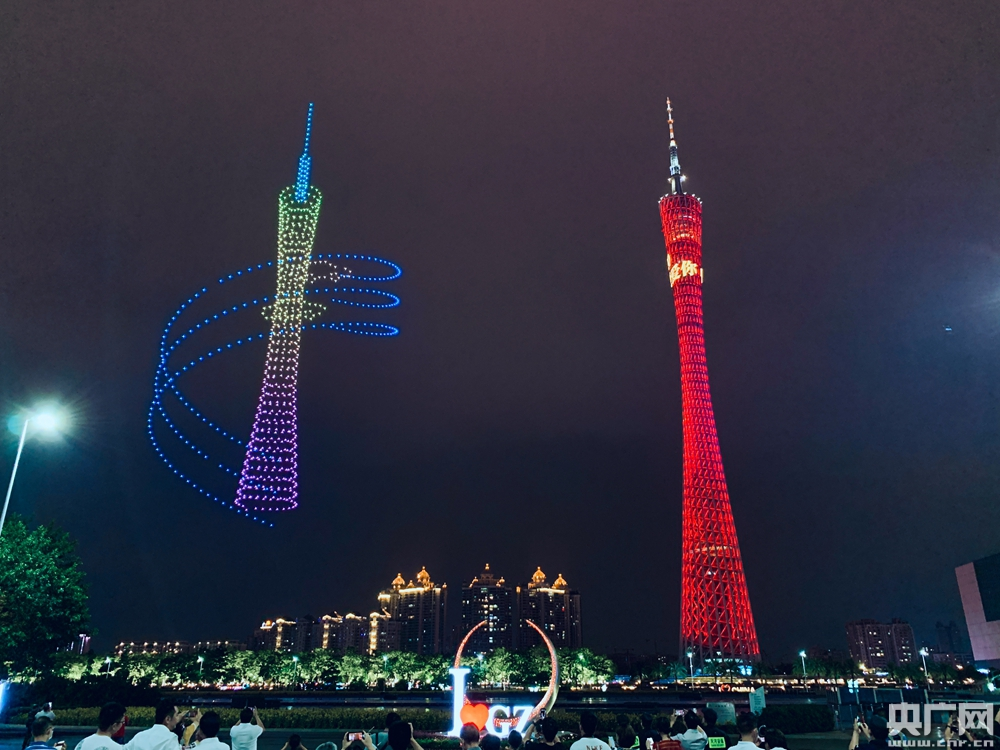
\includegraphics[width=1\linewidth]{Fig/show.jpeg}
				\caption{无人机灯光秀}
		\end{minipage}%
		\begin{minipage}[c]{0.33\textwidth}
				\centering
				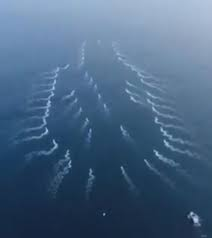
\includegraphics[width=0.8\linewidth]{Fig/AUV_formation.jpeg}
				\caption{\label{}无人船编队}
		\end{minipage}
		\begin{minipage}[c]{0.33\textwidth}
			\centering
			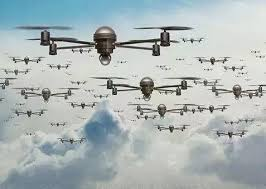
\includegraphics[width=1\linewidth]{Fig/applied_fomation.jpeg}
			\caption{\label{}无人机编队}
		\end{minipage}
	\end{figure}		
\end{frame}

\subsection{国内外研究现状}
\begin{frame}
	\frametitle{多智能体编队控制研究现状}
	\begin{figure}[htbp]
		\centering
		\begin{minipage}[c]{0.5\textwidth} 
			\centering
			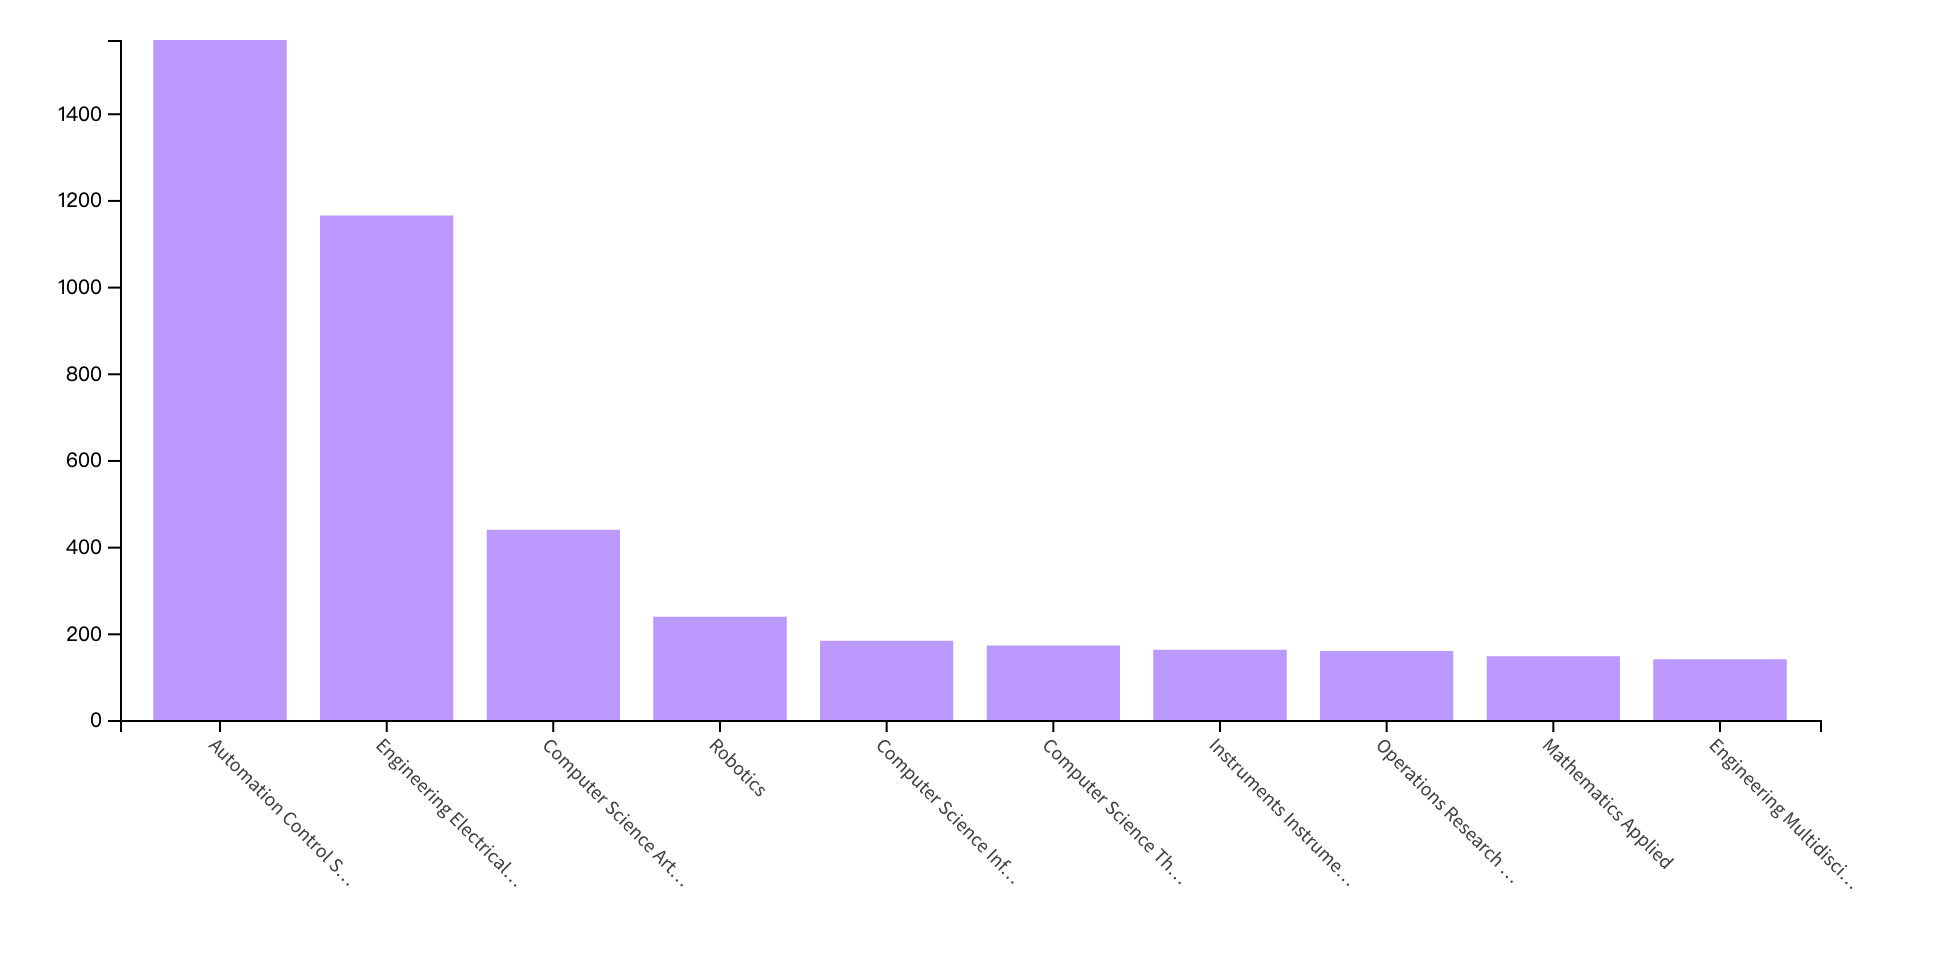
\includegraphics[width=0.8\linewidth]{Fig/formation Control of multi agent _filed.jpg}
			\caption{所属领域:Automation Control Systems,Engineering Electrical Electronic,Computer Science Artificial Intelligence,Robotics}
		\end{minipage}%
		\begin{minipage}[c]{0.5\textwidth}
			\centering
			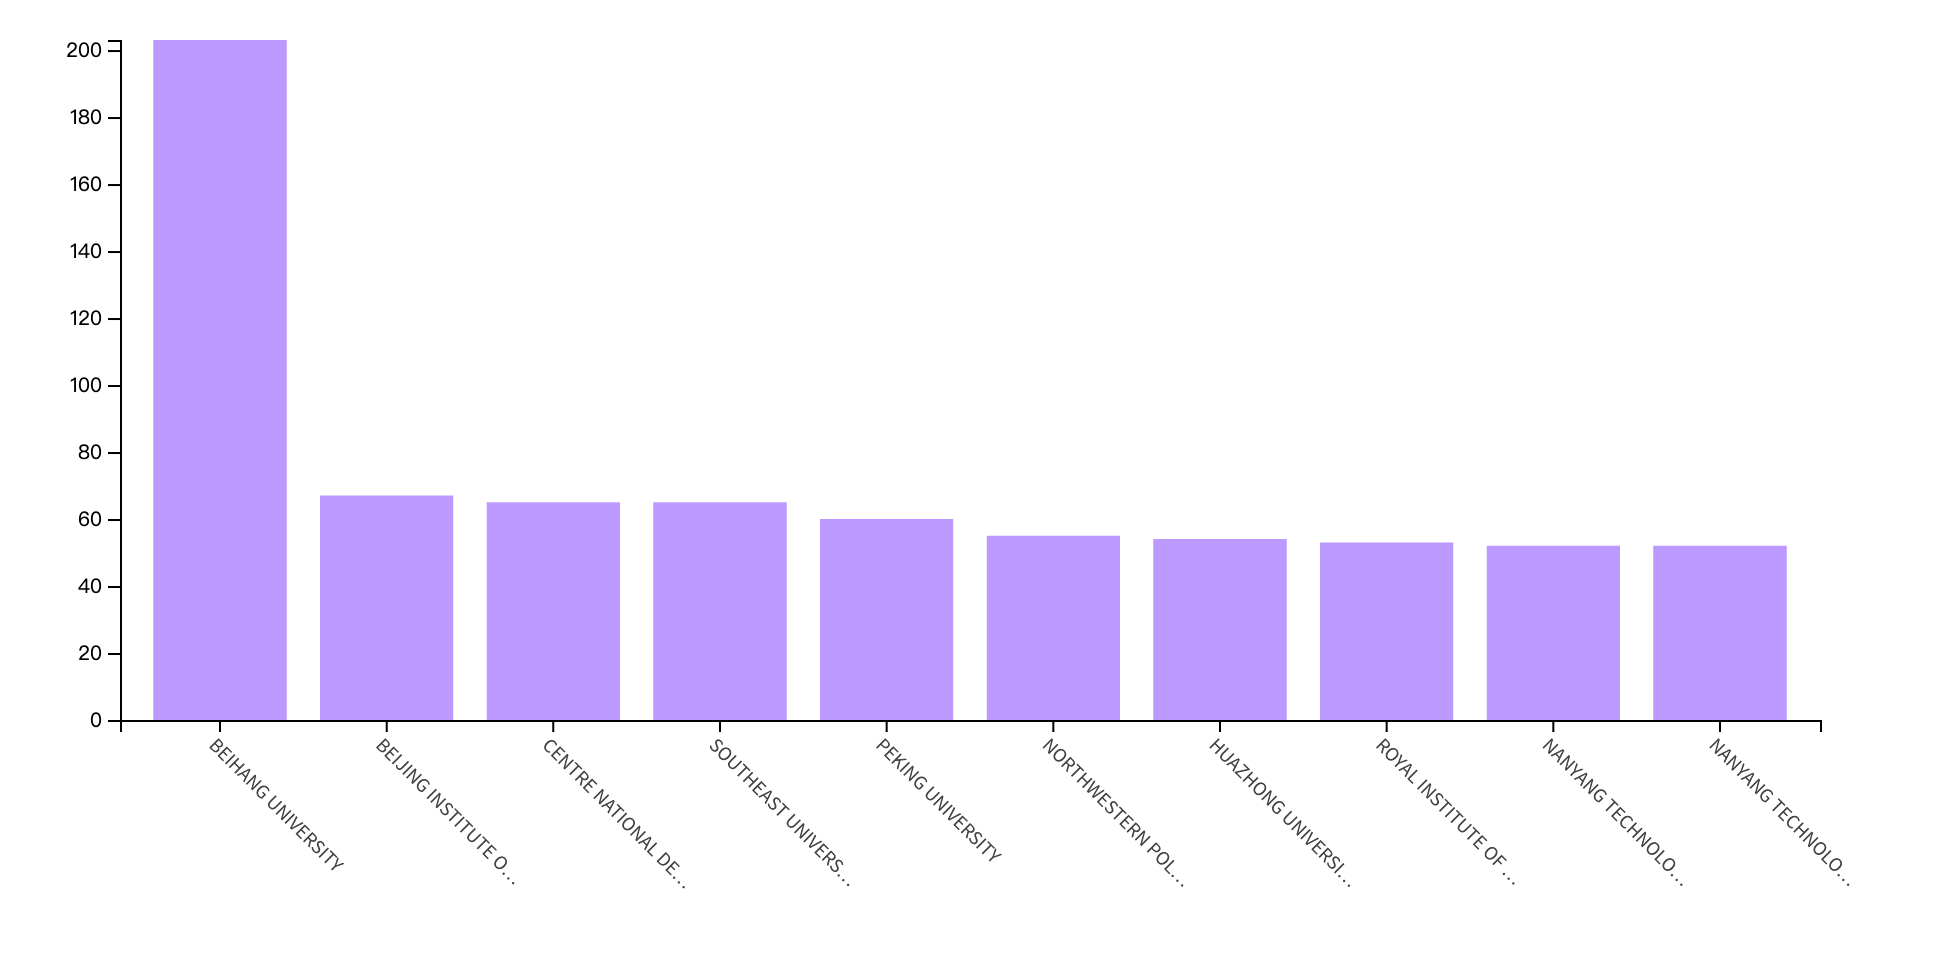
\includegraphics[width=0.8\linewidth]{Fig/formation Control of multi agent _affiliation.jpg}
			\caption{作者单位:北航、北理、法国国家科学研究中心、西工大}
		\end{minipage}
	\end{figure}	
	\begin{figure}[htbp]
		\centering
		\begin{minipage}[c]{0.5\textwidth} 
			\centering
			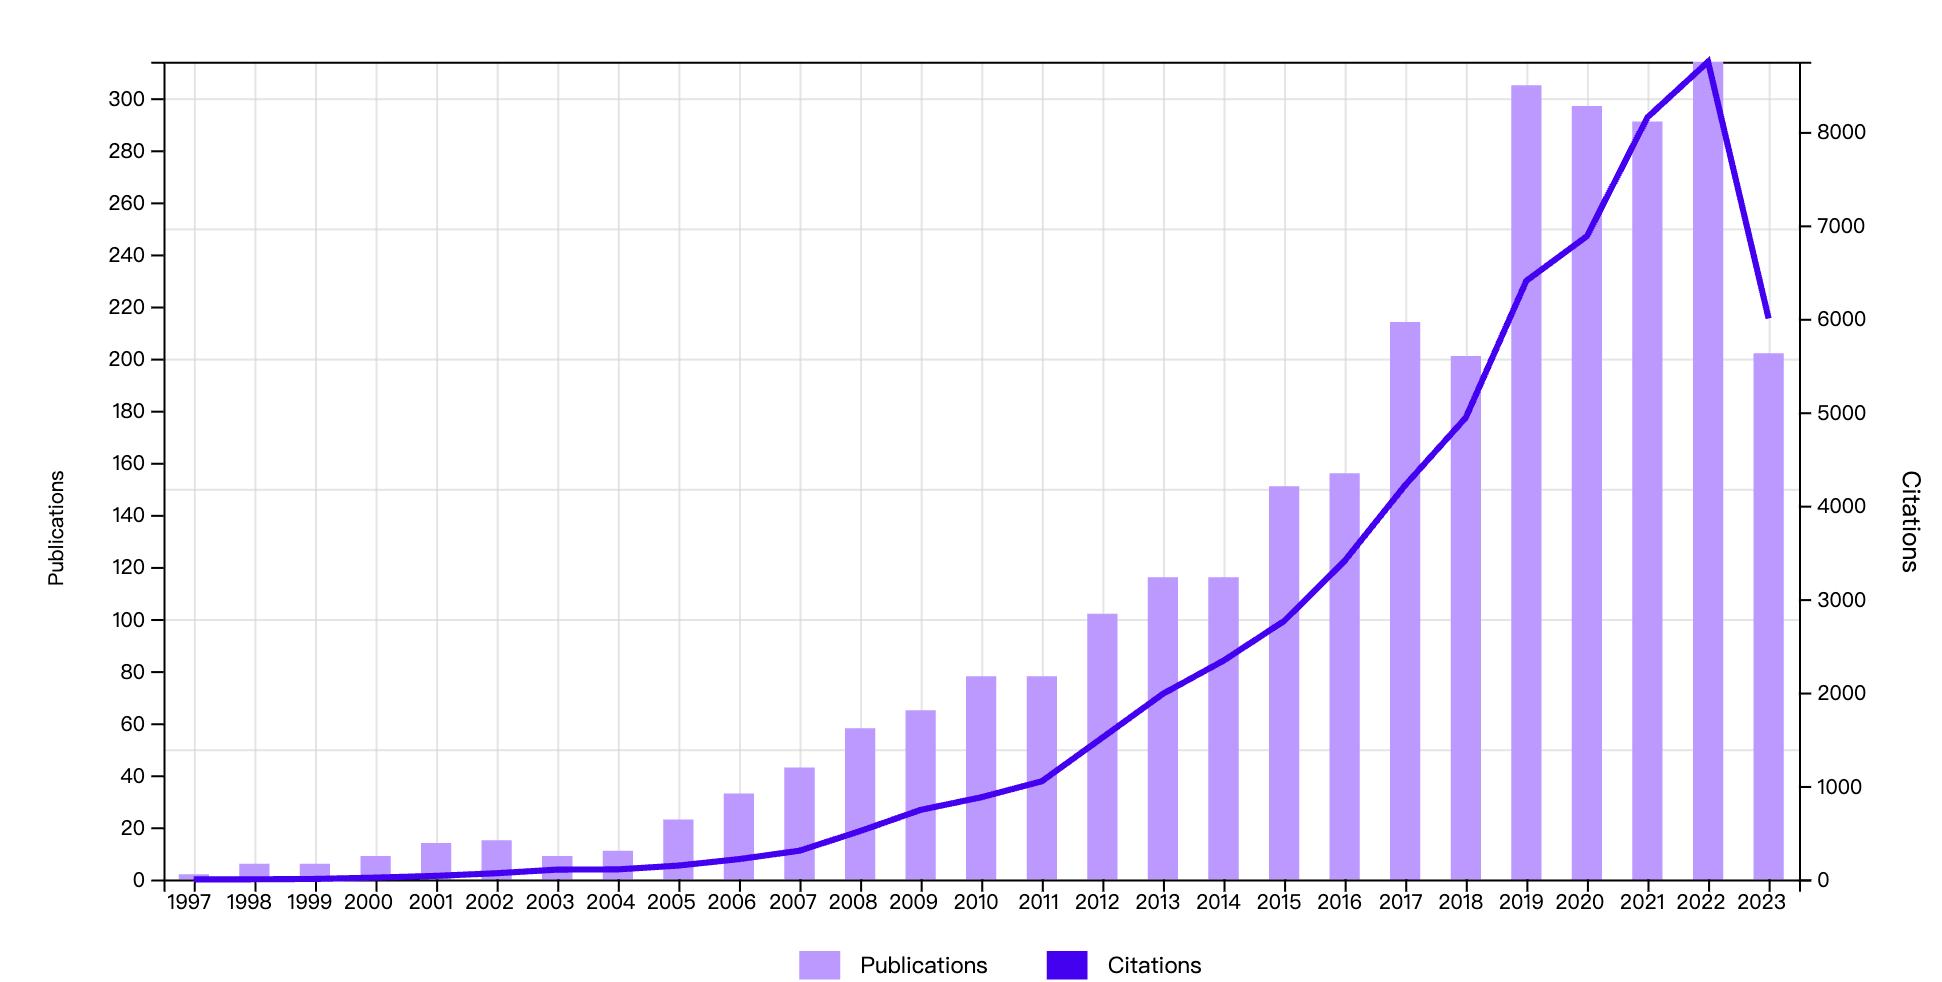
\includegraphics[width=0.8\linewidth]{Fig/formation Control of multi agent _all.jpg}
			\caption{引文数(蓝线)及刊物数(条形)}
		\end{minipage}%
		\begin{minipage}[c]{0.5\textwidth}
			\centering
			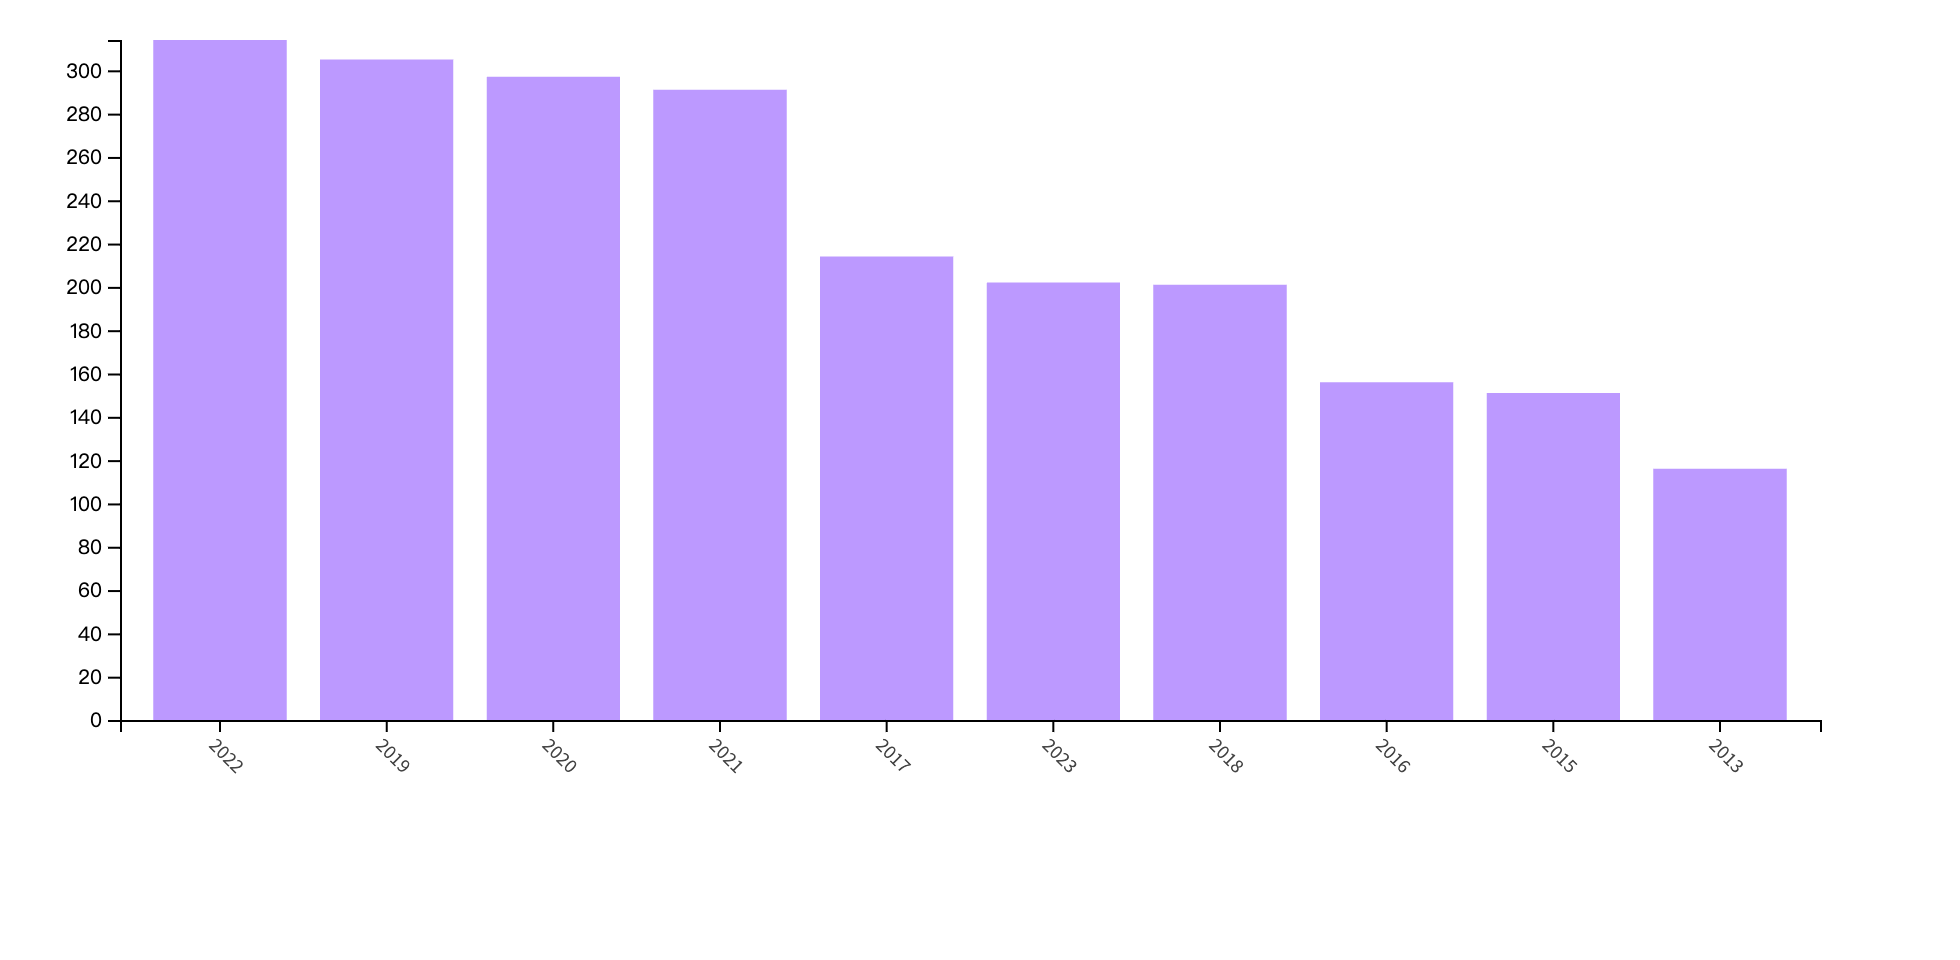
\includegraphics[width=0.8\linewidth]{Fig/formation Control of multi agent _year.jpg}
			\caption{发表年份:2022,2019,2020,2021}
		\end{minipage}
	\end{figure}	
\end{frame}

\begin{frame}
	\frametitle{多智能体编队控制方法分类}
	\begin{itemize}
		\item 根据各智能体之间的信息获取方式划分
		\begin{itemize}
			\item 集中式控制
			\item 分布式控制
		\end{itemize}
		\item 根据智能体信息交互拓扑划分
		\begin{itemize}
			\item 领航跟随法
			\item 基于行为法
			\item 虚拟结构法
		\end{itemize} 
		\item 根据编队目标队形的约束变量划分
		\begin{itemize}
			\item 基于距离 
			\item 基于位置
			\item 基于位移
			\item 基于方位
		\end{itemize}  
	\end{itemize}
\end{frame}

\begin{frame}
	\frametitle{基于方位信息的编队控制研究现状}
	\begin{figure}[htbp]
		\centering
		\begin{minipage}[c]{0.5\textwidth} 
			\centering
			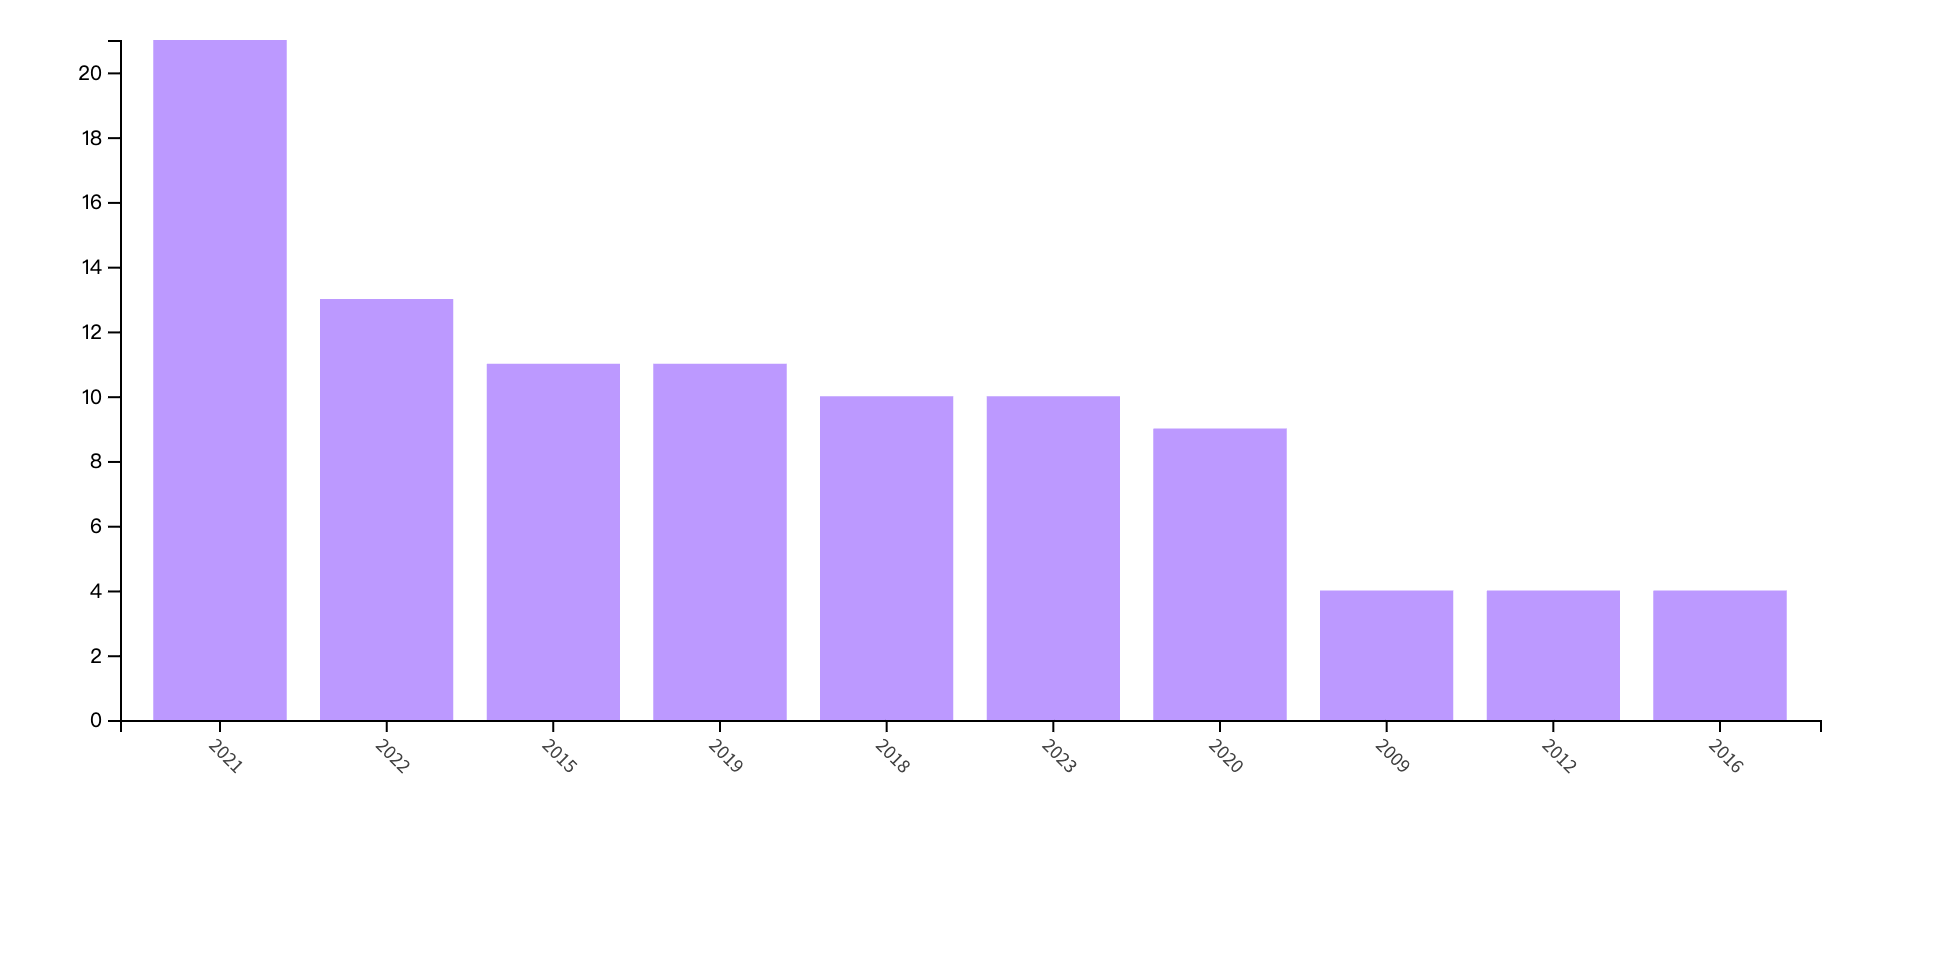
\includegraphics[width=1\linewidth]{Fig/bearing_year.jpg}
			\caption{出版年份:2021,2022,2015,2019}
		\end{minipage}%
		\begin{minipage}[c]{0.5\textwidth}
			\centering
			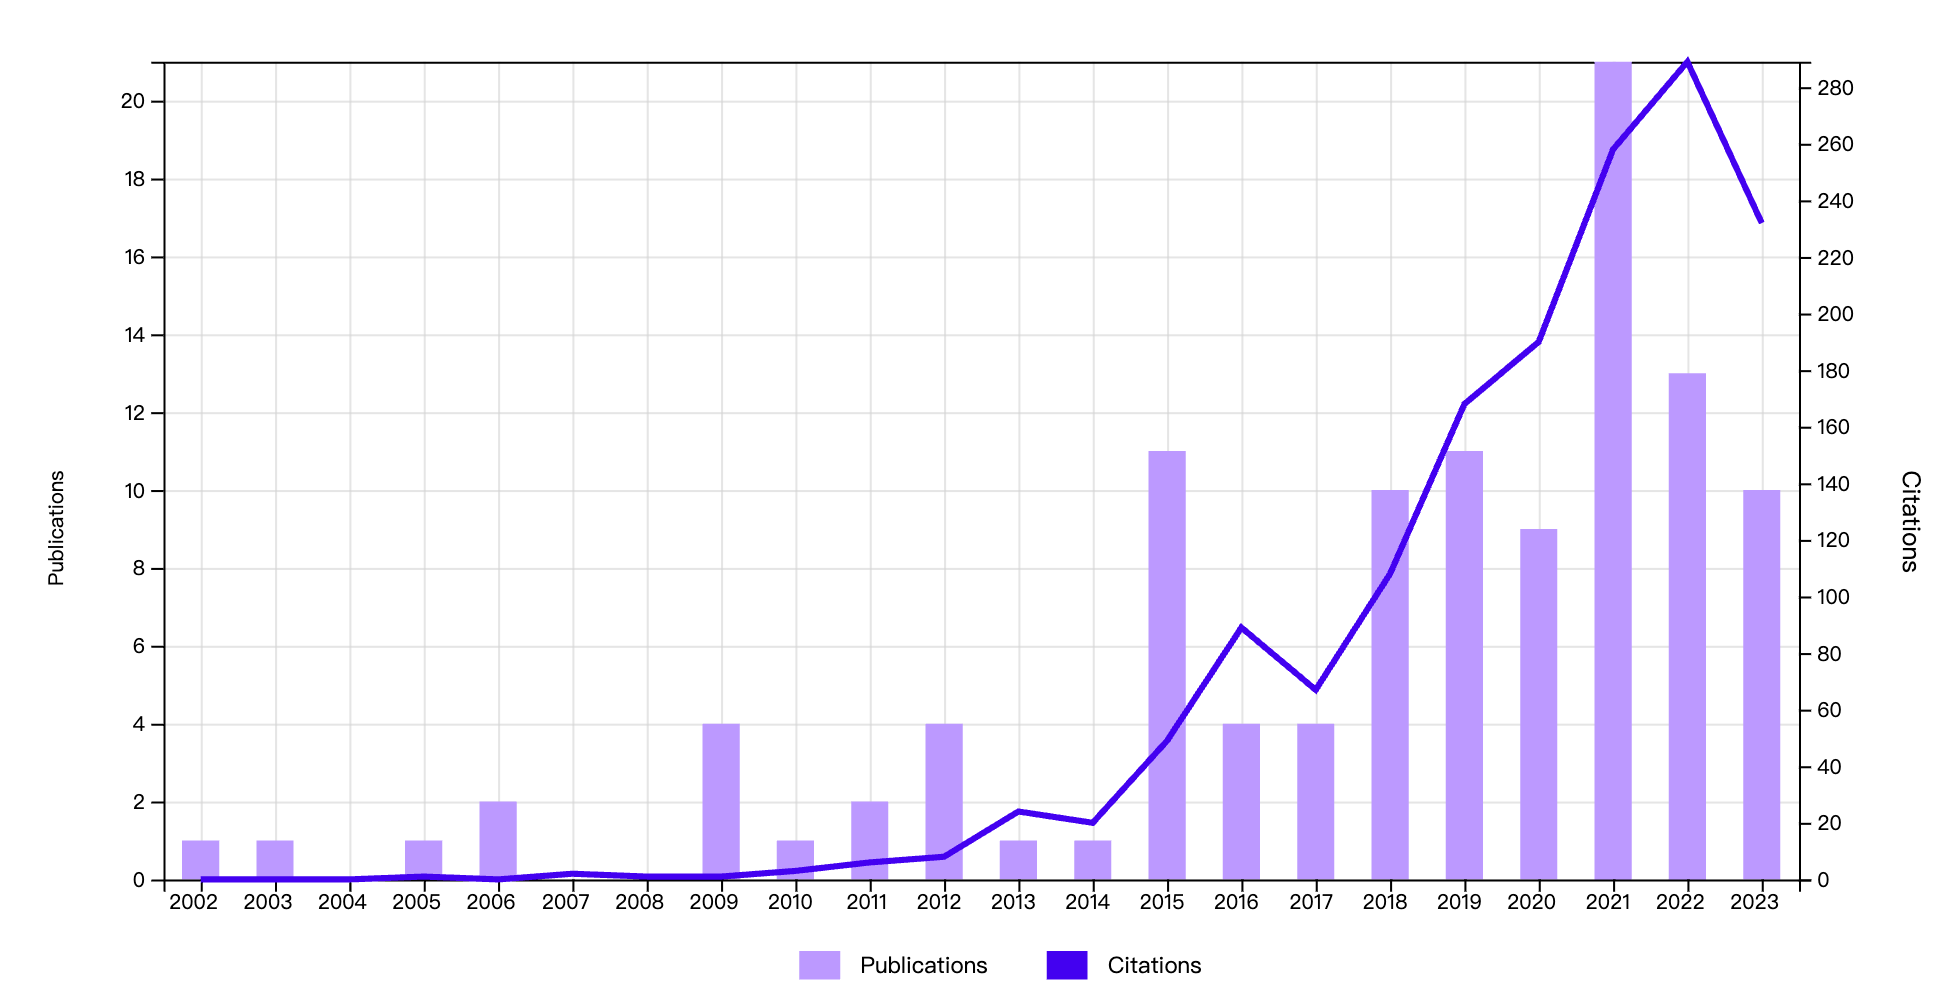
\includegraphics[width=1\linewidth]{Fig/bearing_all.jpg}
			\caption{引文数(蓝线)及刊物数(条形)}
		\end{minipage}
	\end{figure}	
	\begin{figure}[htbp]
		\centering
		\begin{minipage}[c]{0.5\textwidth} 
			\centering
			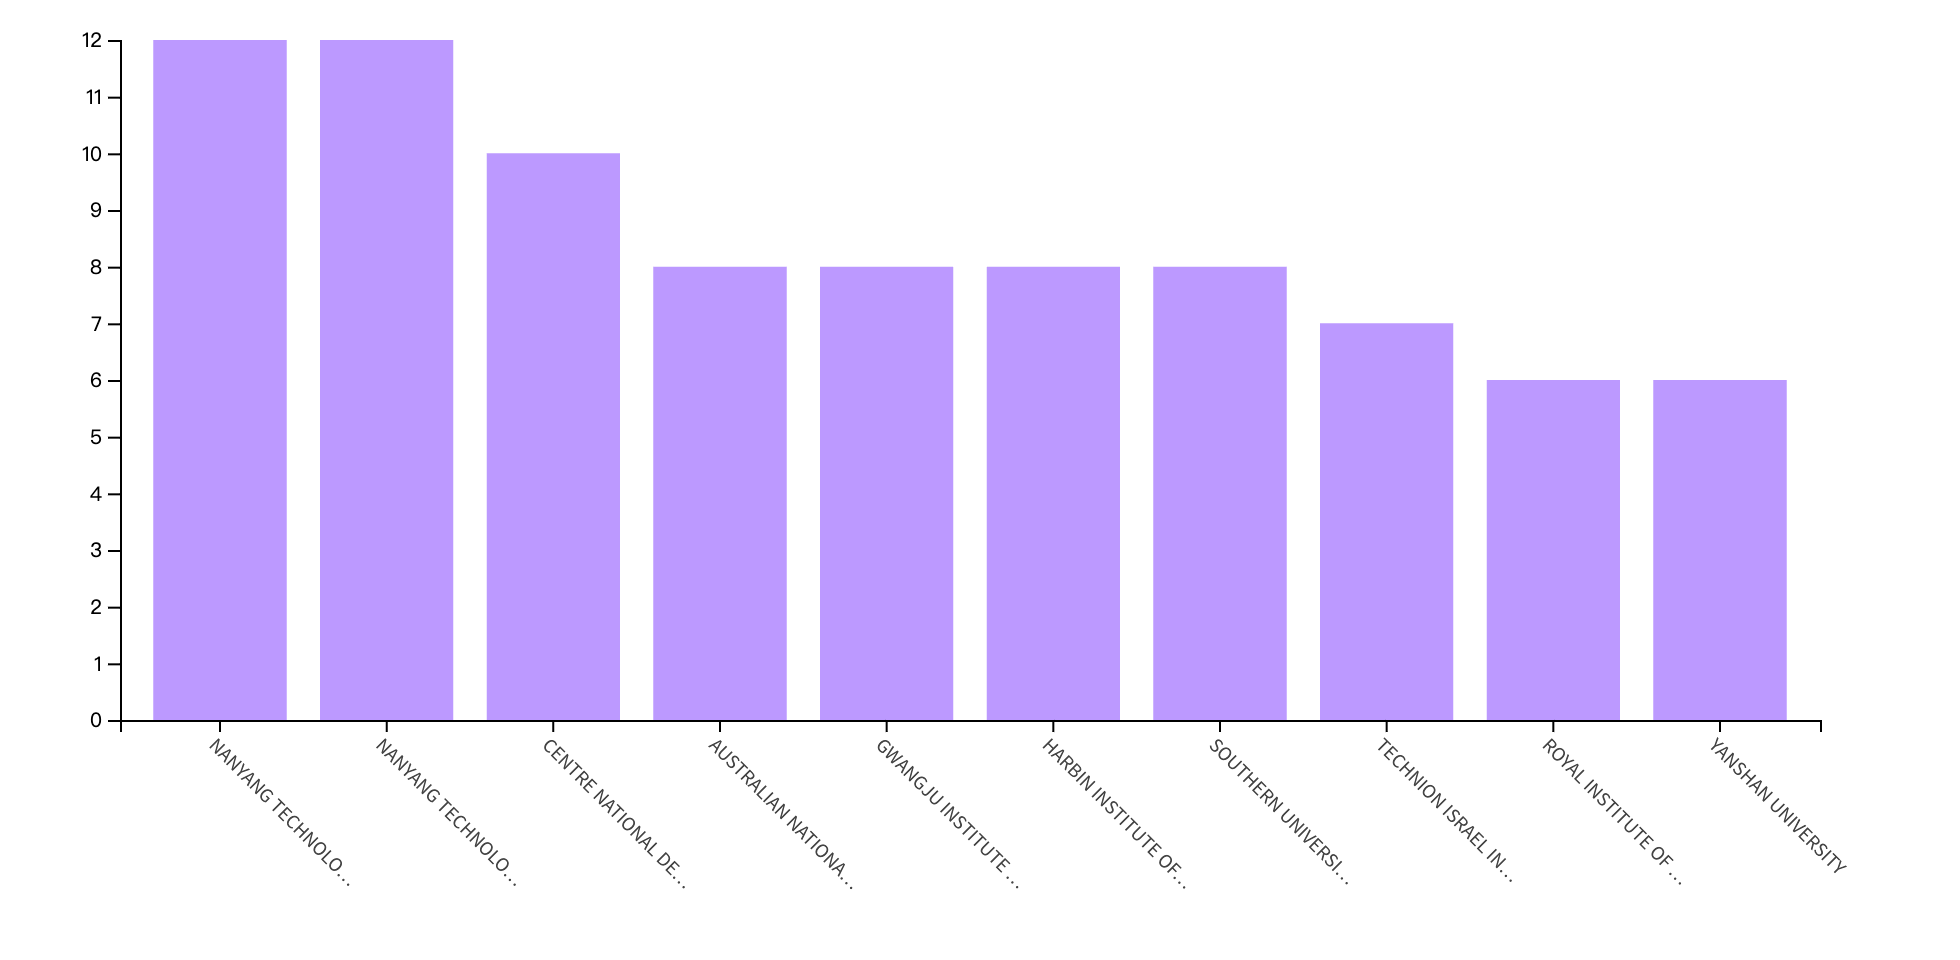
\includegraphics[width=1\linewidth]{Fig/bearing_affiliation.jpg}
			\caption{作者单位:NTU,法国国家科学研究中心,ANU,哈工大}
		\end{minipage}%
		\begin{minipage}[c]{0.5\textwidth}
			\centering
			
		\end{minipage}
	\end{figure}	
\end{frame}


\section{研究方案}
\subsection{基于xxx的分布式编队控制}
\begin{frame}
	\frametitle{研究动机}
	\begin{itemize}
		\item  xxxxxxxxxxxxxxxxxxxxx
		\item xxxxxxxxxxxxxxxxxxxxx
		\item $SE(2)$以及$SE(n)$中的方位刚性理论已经成熟。
	\end{itemize}
	\begin{figure}[htbp]
		\centering
			\centering
			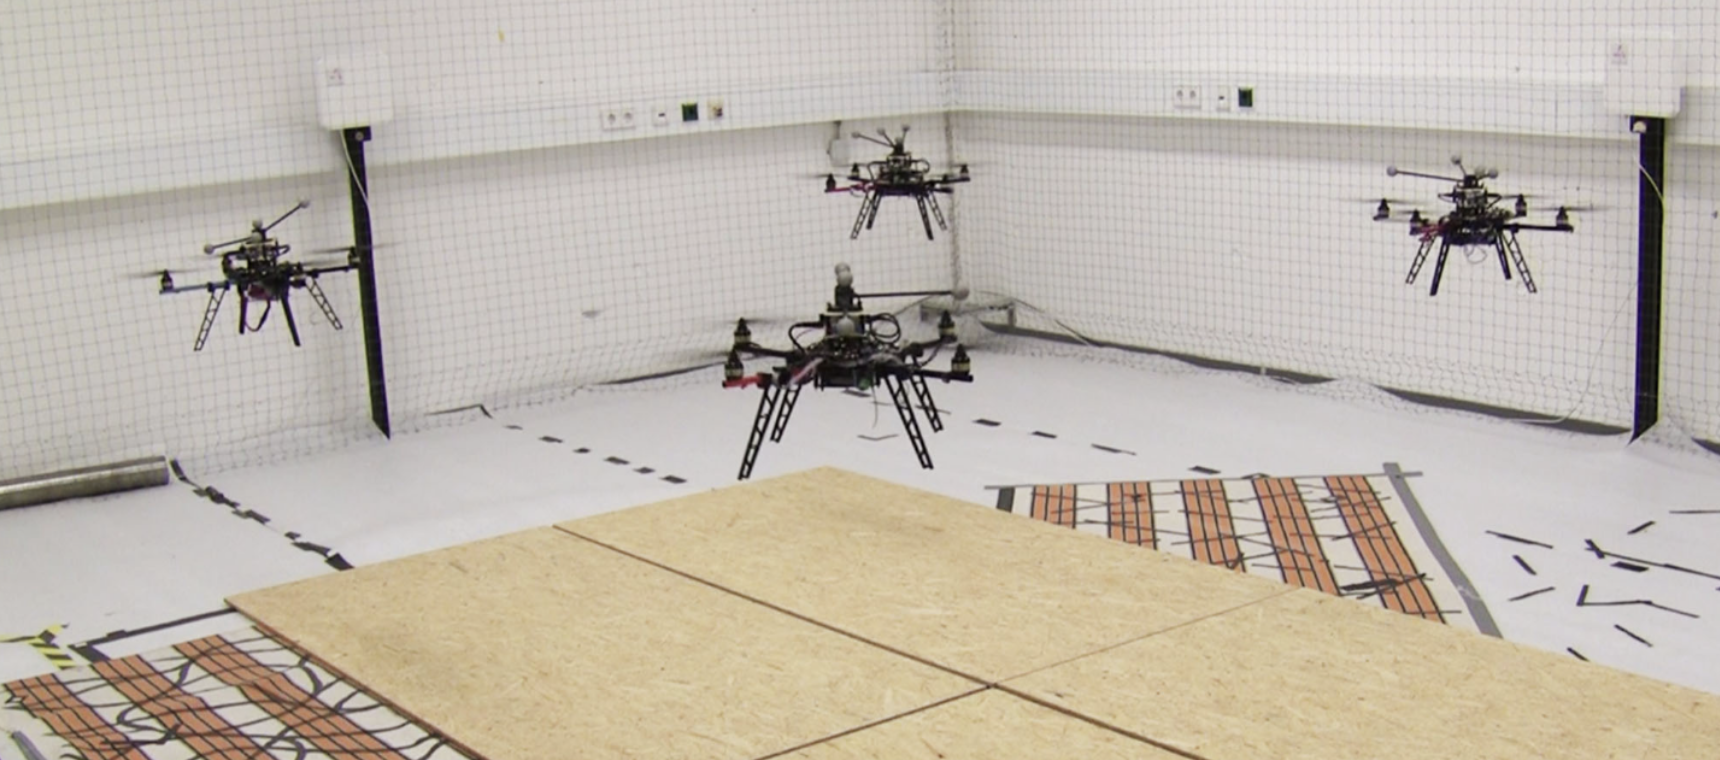
\includegraphics[width=0.8\linewidth]{Fig/f5.png}
			\caption{室内无人机群}
	\end{figure}	
\end{frame}

\begin{frame}
	\frametitle{问题阐述}
	\begin{itemize}
		\item 由无人机的微分平坦性,其状态由$\bm{q}_i=(\bm{p_i}, {\psi}_i) \in \mathbb{R}^3\times\mathcal{S}^1$描述。
		\item 定义局部坐标系下的方位函数$\bm{\beta}_{\mathcal{G}}(\bm{q})$,为由$\bm{\beta}_{ij}$堆叠得到的列向量。
		\item 控制目标是使方位误差$\bm{e}(\bm{q}) =\bm{\beta}_{\mathcal{G}}(\bm{q})   −  \bm{\beta}_{\mathcal{G}}(\bm{q}_{d})  $收敛至零。
		
	\end{itemize}
	\quad
	\quad
	\begin{equation}
		\left.\left(\begin{array}{c}\dot{\bm{p}}_i\\\dot{\psi}_i\end{array}\right.\right)=\left(\begin{array}{cc}R_i&0\\\bm{0}&1\end{array}\right)\left(\begin{array}{c}\bm{u}_i\\w_i\end{array}\right)
		\label{equ1}
	\end{equation}
	\quad
	\quad
	\begin{equation}
		\bm{\beta}_{ij}=\bm{R}_{i}^{T}\frac{\bm{p}_{j}-\bm{p}_{i}}{\|\bm{p}_{j}-\bm{p}_{i}\|}\in\mathbb{S}^{2}.
	\end{equation}
	\quad
	\quad
	问题阐述为:针对模型为式\eqref{equ1}的系统,如何利用方位测量信息$\bm{\beta}_{ij}$,设计控制器使得$\bm{e}(\bm{q}) \to \bm{0}$。
\end{frame}

\begin{frame}
	\frametitle{研究方法}
	\begin{itemize}
		\item  定义代价函数$J(\bm{q})=\|   \bm{\beta}_{\mathcal{G}}(\bm{q})   − \bm{\beta}_{\mathcal{G}}(\bm{q}_{d})    \|^{2}/{2}$。控制问题变为求解代价函数是$J(\bm{q})$的最优化问题
		\item xxxxxxxxxxxxxxxxxxxxx。
		\item xxxxxxxxxxxxxxxxxxxxx。
	\end{itemize}
	\begin{equation}
		\left.\left[\begin{array}{c}\dot{\bm{p}}\\\dot{\psi}\end{array}\right.\right]=-k_c\nabla_{\bm{q}}J(\bm{q})=k_c\mathcal{\bm{B}}_{\mathcal{G}}^{\mathcal{W}}(\bm{q})^{T} \bm{\beta}_{\mathcal{G}}(\bm{q}_{d})
	\end{equation}
	\begin{equation}
		\left.\left\{\begin{array}{rcl}\bm{u}_i&=&-k_c\sum_{(i,j)\in\mathcal{E}}\bm{P}_{ij}\bm{\beta}_{ij}^d+k_c\sum_{(j,i)\in\mathcal{E}}{}^i\bm{R}_j\bm{P}_{ji}\bm{\beta}_{ji}^d\\\\w_i&=&k_c\sum_{(i,j)\in\mathcal{E}}\bm{\beta}_{ij}^T\bm{S}\bm{\beta}_{ij}^d\end{array}\right.\right.
		\label{equ13}
	\end{equation}
\end{frame}


\subsection{基于xxxxx的四旋翼无人机编队}


\begin{frame}
	\frametitle{研究动机}
	\begin{itemize}
		\item 仅考虑无人机$\mathbb{R}^3\times\mathcal{S}^1$中的运动学模型,忽略了欠驱动特性。
		\item xxxxxxxxxxxxxxxxxxxxx
		\item xxxxxxxxxxxxxxxxxxxxx
	\end{itemize}
	\begin{figure}[htbp]
		\centering
			\centering
			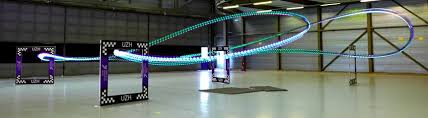
\includegraphics[width=1\linewidth]{Fig/MPC.jpeg}
			\caption{State of The Art MPC}
	\end{figure}

\end{frame}

\begin{frame}
	\frametitle{问题阐述}
	\begin{itemize}
		\item  xxxxxxxxxxxxxxxxxxxxx
	\end{itemize}
	\begin{minipage}[c]{0.5\textwidth} 
		\begin{figure}[H]
			\centering
			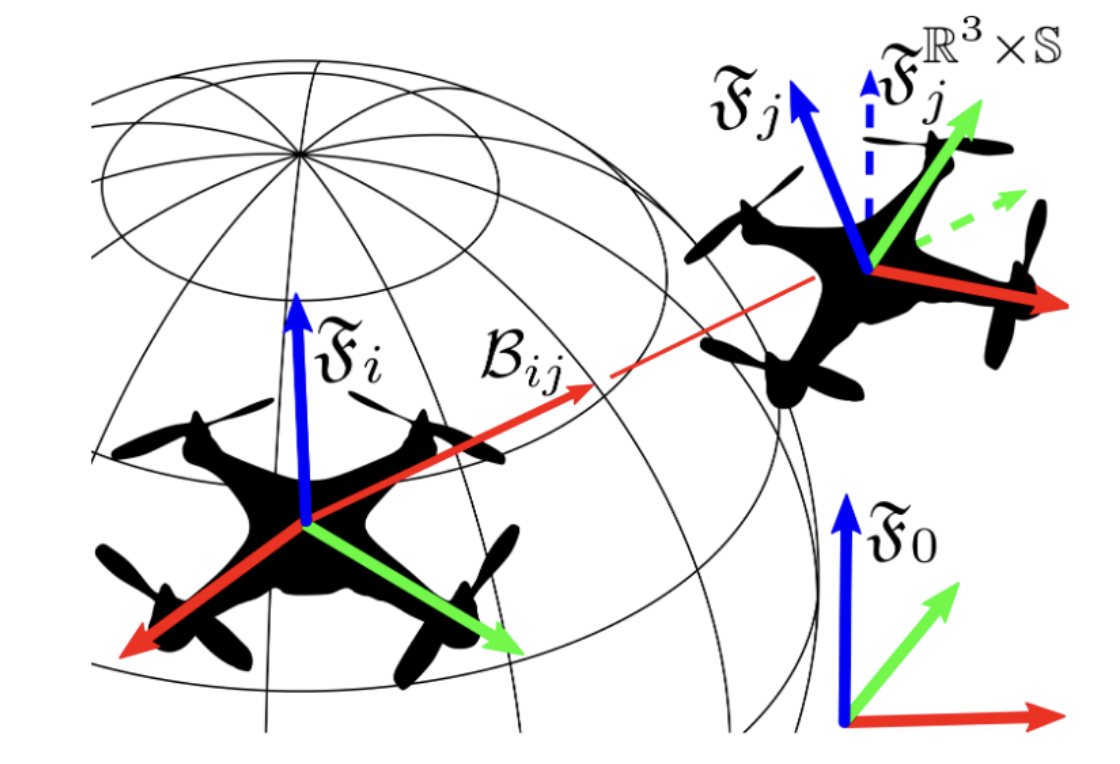
\includegraphics[width=1\linewidth]{Fig/f10.png}
			\caption{坐标系关系}
		\end{figure}
	\end{minipage}%
	\begin{minipage}[c]{0.5\textwidth}
		\centering
		\begin{equation}
			\begin{aligned}
				&\min_{\bm{u}} \sum_{i=1}^{N_{p}}{\cal O}(\bm{q},\bm{q}^{d},{\bm{u}},\Delta t)  \\
				&\bm{s.t.} \bm{\underline{u}}\leq\bm{u}\leq\bm{\bar{u}}  \\
				&{\mathcal{C}}_{eq}(\bm{q},\bm{u})=0 \\
				&{\mathcal{C}(\bm{q},\bm{u})}{{}\leq0}
			\end{aligned}
			\label{equ_mpc}
		\end{equation}
	\end{minipage}
	
\end{frame}

\begin{frame}
	\frametitle{研究方法}
	\begin{itemize}
		\item  目标函数可以是$\bm{q}_i(t)$、方位 $	\bm{\beta}_i(t) $和输入 $\bm{u}_i(t) $的函数,以同时实现:
		\begin{itemize}
			\item xxxxxxxxxxxxxxxxxxxxx
			\item xxxxxxxxxxxxxxxxxxxxx
		\end{itemize}
		\item xxxxxxxxxxxxxxxxxxxxx,多目标优化问题:$\mathcal{O}_{i}=\mathcal{O}_{\boldsymbol{\beta}i}+w\mathcal{O}_{\mathfrak{M}i}$
		\item 除了与无人机本身有关的约束外,还考虑视线约束,碰撞约束等。
	\end{itemize}
	\begin{equation}
		\begin{aligned}
			&\begin{aligned}\underline{f}_i&\leq&f_i&\leq\bar{f_i}\end{aligned} \\
			\underline{\boldsymbol{\omega}}_{xy,i}& \leq\boldsymbol{\omega}_{xy,i}\leq\bar{\boldsymbol{\omega}}_{xy,i}  \\
			\underline{\omega}_{z,i}& \leq\left.\omega_{z,i}\right.\leq\bar{\omega}_{z,i} 
		\end{aligned}
	\end{equation}
\end{frame}

\subsection{仿射编队机动控制}
\begin{frame}
	\frametitle{研究动机}
	\begin{itemize}
		\item  仿射编队机动控制(Affine Formation Maneuver Control)可以同时实现队形收敛和编队机动。
		\item 仿射变换可对应空间中的平移、旋转、缩放、剪切或上述组合。
		\item 应力矩阵对于编队构型的任何仿射变换的不变性。可作为研究编队机动的工具。
	\end{itemize}
	\begin{figure}[H]
		\centering
		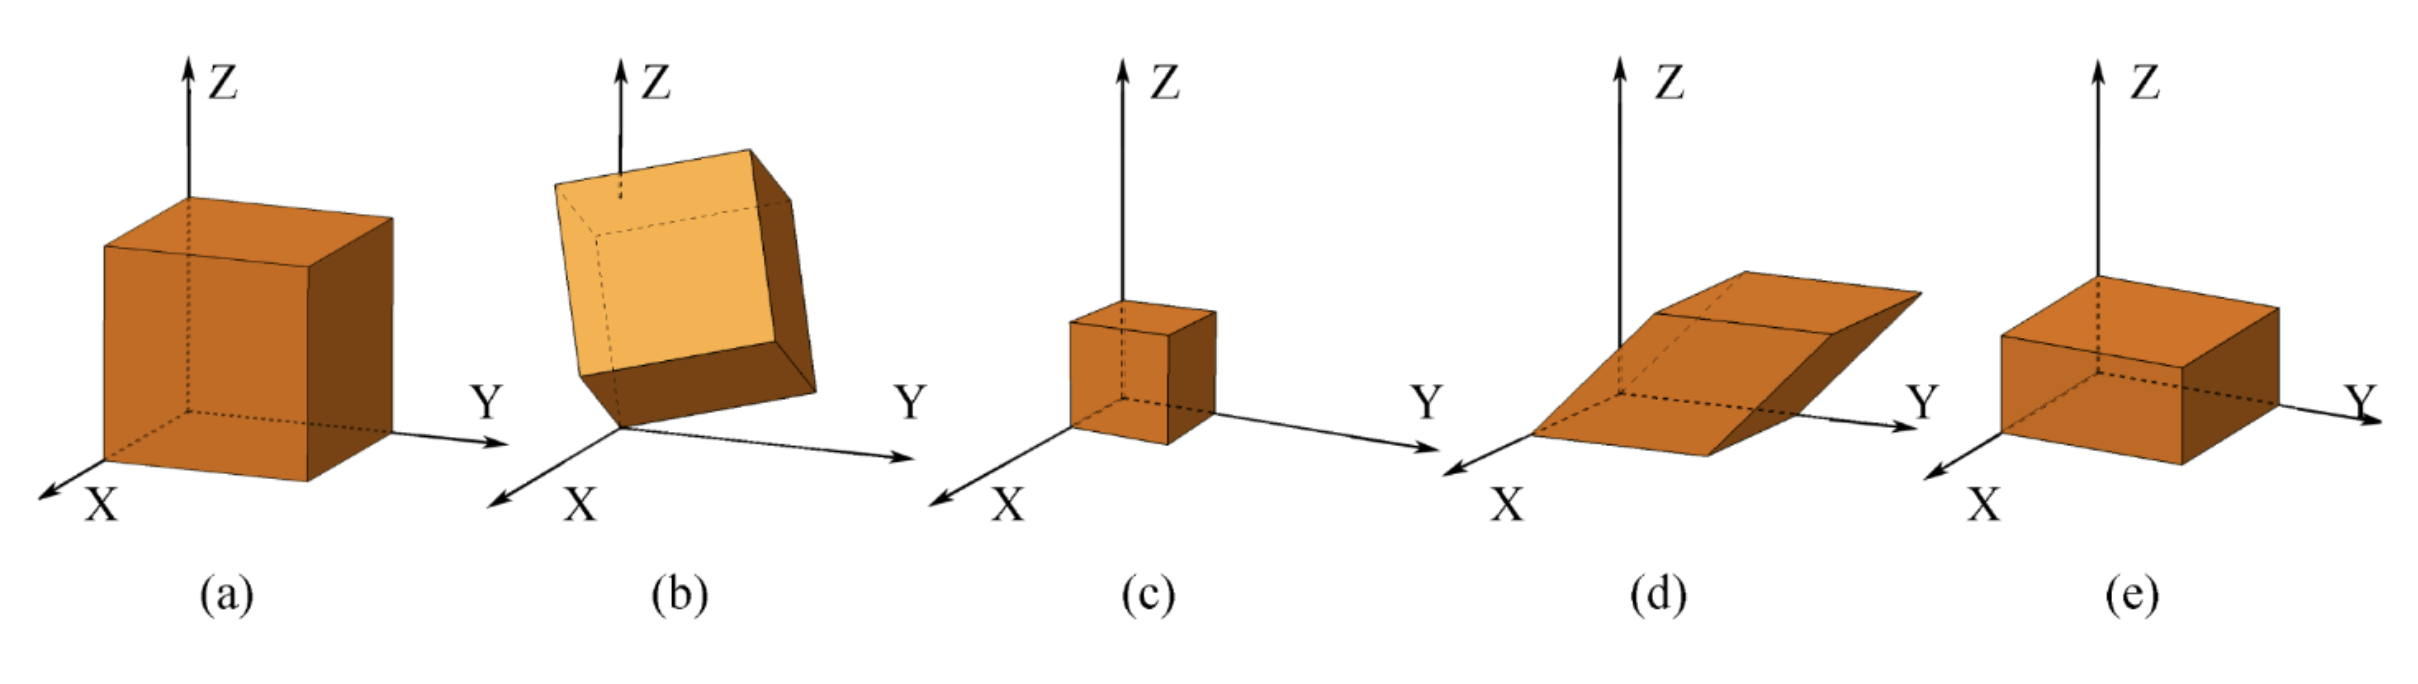
\includegraphics[width=1\linewidth]{Fig/affine.png}
		\caption{$\mathbb{R}^3$空间中仿射变换:(a)初始状态 (b)旋转 (c)缩放 (d)剪切 (e)平移}
	\end{figure}
\end{frame}

\begin{frame}
	\frametitle{问题阐述}
	\footnotesize
	\begin{alertblock}{\footnotesize 假设 1} 
		对标称编队$\left(\mathcal{G},  \bm{r}\right)$,假设$\{r_i\}_{i=1}^n$ 仿射张成 $\mathbb{R}^d$ 。
	\end{alertblock}
	\begin{alertblock}{\footnotesize 假设2} 
		假设标称编队$\left(\mathcal{G},\bm{r}\right)$具有半正定应力矩阵$\Omega$,且满足$\mathrm{rank}(\Omega)=n-d-1$。
	\end{alertblock}
	\begin{alertblock}{\footnotesize 假设3} 
		假设标称编队$\left(\mathcal{G},  \bm{r}\right)$ 是由领导者仿射定位的。
	\end{alertblock}
	\normalsize
	根据代数图论的引理,三个假设最终保证$\bar{\Omega}_{ff}$ 是正定的,且仿射像空间$\mathcal{A}(r)$和应力矩阵的零空间有一定联系:
	\footnotesize
	\begin{lemma}
		若假设2成立,则以下条件等价:

		1)$\{r_i\}_{i=1}^n$仿射张成$\mathbb{R}^d$。

		2)$Null(\Omega\otimes I_d)= \mathcal{A}(r)$

		3)$Null(\Omega)=\mathrm{Col}(\bar{P}(r))$
	\end{lemma}
	
\end{frame}
\begin{frame}
	\frametitle{问题阐述}
	\begin{itemize}
		\item  三个假设隐含:$\bar{\Omega}_{ff}$ 是正定的。
		\quad
		\item xxxxxxxxxxxxxxxxxxxxx。
		\item xxxxxxxxxxxxxxxxxxxxx
	\end{itemize}

	xxxxxxxxxxxxxxxxxxxxx。 

	\quad
	\quad
	\begin{equation}
		\left.\bar{\Omega}=\left[\begin{array}{cc}\bar{\Omega}_{\ell\ell}&\bar{\Omega}_{\ell f}\\\bar{\Omega}_{f\ell}&\bar{\Omega}_{ff}\end{array}\right.\right]
	\end{equation}

	\begin{equation}
		p^*(t)=[I_n\otimes A(t)]r+\mathbf{1}_n\otimes b(t)
	\end{equation}

	\begin{equation}
			\mathcal{A}(r)=\left\{p\in\mathbb{R}^{dn}:p=(I_n\otimes A)r+1_n\otimes b, A\in\mathbb{R}^{d\times d},b\in\mathbb{R}^d\right\}
	\end{equation}
\end{frame}
\begin{frame}
	\frametitle{研究方法}
	\begin{itemize}
		\item xxxxxxxxxxxxxxxxxxxxx。
		\item xxxxxxxxxxxxxxxxxxxxx。
		\item xxxxxxxxxxxxxxxxxxxxx。
	\end{itemize}
\end{frame}


% \begin{frame}
% 	\frametitle{数学环境}
% 	% create a basic block
% 	\begin{block}{Basic block title} 
% 		Basic block contents.
% 	\end{block}
	
% % create an example block    
% 	\begin{exampleblock}{Example block title} 
% 		Example block contents.
% 	\end{exampleblock}
	
% % create an alert block  
% 	\begin{alertblock}{Alert block title} 
% 		Alert block contents.
% 	\end{alertblock}
% 	\begin{theorem} ... \end{theorem}
% \end{frame}

% \begin{frame}
% 	\frametitle{数学环境}
% 	\begin{definition} ... \end{definition}
% 	\begin{proof} ... \end{proof}
% 	\begin{lemma} ... \end{lemma}
% 	\begin{corollary} ... \end{corollary}
% 	\begin{example} ... \end{example}
% \end{frame}


\section{研究条件与基础}
\subsection{研究条件}
\begin{frame}
	\frametitle{研究条件}
\end{frame}

\subsection{已取得的主要成果}
\begin{frame}
	\frametitle{已取得的主要成果}
	\begin{itemize}
		\item 
	\end{itemize}

\end{frame}

\LogoOff

% 记得要用{} 括号把这个frame给包起来
{
% 这是关键代码
% 透明度的修改在于:\tikz[overlay,remember picture]\node[opacity=0.3]   中的opacity这个参数,越小越透明
\usebackgroundtemplate{\tikz[overlay,remember picture]\node[opacity=0.08]at (current page.center){
\includegraphics[width=0.5\paperwidth]{2.jpeg}};}

% 这些注释代码可以参考一二
% \tikz[overlay,remember picture]\node[opacity=0.15]at (current page.center)
% \usebackgroundtemplate{\tikz\node[opacity=0.3]{\includegraphics[width=\paperwidth,height=\paperheight]{figs/thank-you.png}};}%

\begin{frame}
    \begin{center}
    \Huge 
    {
        % \fontfamily{comic}\selectfont 
	    感谢聆听!敬请批评指正!
    }
    \end{center}
\end{frame}

}
\end{document}

